\documentclass{article}

\usepackage[english]{babel}
\usepackage{microtype}
\usepackage{graphicx}
\usepackage{wrapfig}
\usepackage{enumitem}
\usepackage{fancyhdr}
\usepackage{amsmath}
\usepackage{index}
\usepackage{hyperref}
\usepackage[margin=1.0in]{geometry}
\usepackage{float}

\begin{document}
\title{HW4 Bonus: HTTP Performance Analysis}
\author{Dowland Aiello}
\date{}

\maketitle
\fancyhf{}

\section{About}

My bonus extension to the CSE 333 hw4 lab implements, and presents the
findings, of a testing utility written in Rust that determines the maximum
throughput in \emph{requests per second}, \emph{bytes per second}, and
\emph{latency per connection} as a function of the length of a query submitted
to the http333d web server. The tool uses \textbf{httperf} and the
\textbf{plotters} library written in Rust to automate the process of running
these tests. The source code used to generate these tests is available
\href{https://github.com/dowlandaiello/hw4-analysis}{\textbf{here}}.

\section{Findings}

\begin{figure}[h]
	\begin{center}
	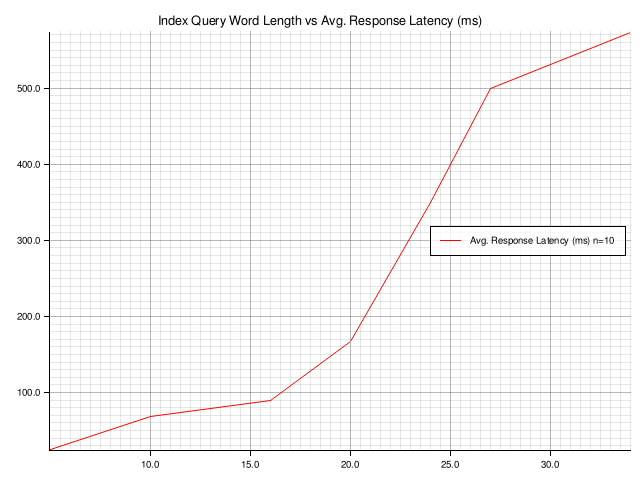
\includegraphics[width=.3\linewidth]{media/multisampled_latency.png}
	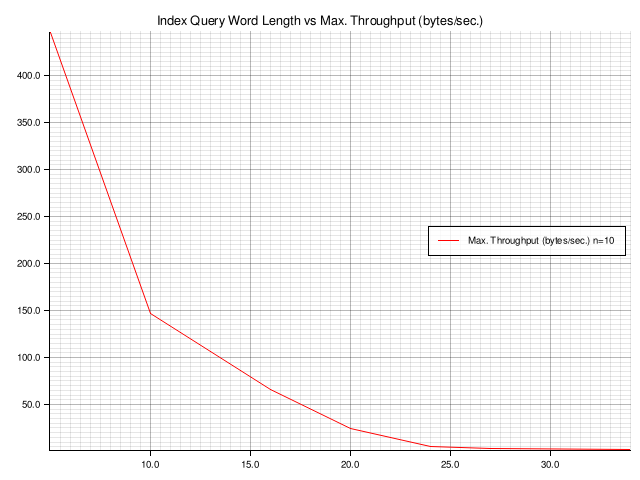
\includegraphics[width=.3\linewidth]{media/multisampled_throughput_bytes.png}
	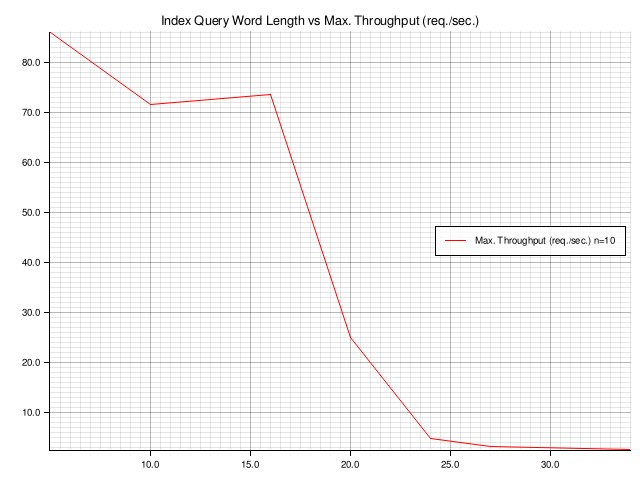
\includegraphics[width=.3\linewidth]{media/multisampled_throughput_requests.png}
		\caption{Request latency, and throughput (req./s, KB/s) as a function of query length}
	\end{center}
\end{figure}

\bigbreak{}

As is demonstrated in the 3 images above, the performance of the http333d
server decreases exponentially as the length of a requested query increases.
These results suggest that a compensating mechanism must be implemented in the
http333d server to allow long, but frequent queries to place less of a
bottleneck on the performance of the server. One such mechanism could be
secondary caching in a least-recently-used manner, prioritized by query length,
where such queries are persisted to memory, and evicted once they are no longer
common. However, an alternative approach where the most frequently used
branches along nested query rankings are cached instead (e.g., words like,
``a'') would be better suited for easing this bottleneck.

The efficacy of this alternative approach is suggested by the following results
from the same testing program, with a dictionary of increasingly common words:

\begin{figure}[t]
	\begin{center}
	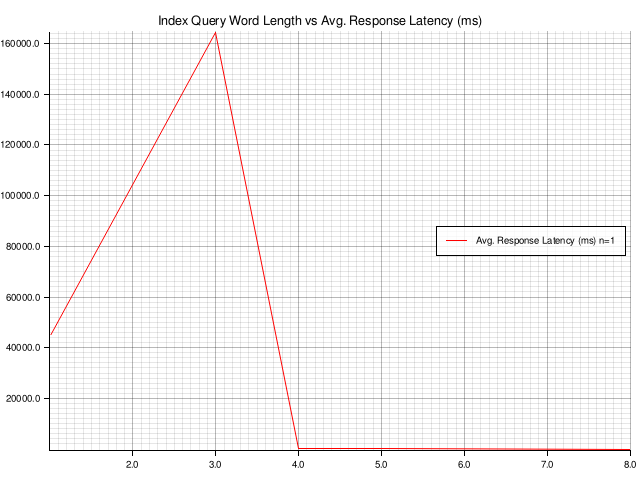
\includegraphics[width=1\linewidth]{media/big_dictionary.png}
		\caption{Shorter queries were correlated with exponentially larger response latency times than queries that used longer words.}
	\end{center}
\end{figure}

\end{document}
